\documentclass[11pt]{article}

\usepackage[margin=2cm]{geometry}

\usepackage{graphicx}

\usepackage{booktabs}

\usepackage{hyperref}

\usepackage[T1]{fontenc}

\usepackage[utf8]{inputenc}

\title{Comparacion del foco textil estricto Santa Ana 2026}

\author{Proyecto Atoyac - salida reproducible}

\date{\today}

\begin{document}

\maketitle

\section{Objetivo}

Este documento compara directamente cuatro conjuntos para Santa Ana Xalmimilulco: el foco textil estricto 2026, el filtrado prioritario DENUE 2026, la capa MH filtrada y la union previa construida en la auditoria. La comparacion se hace por ID DENUE cuando existe; los puntos MH sin ID se mantienen como casos auditables separados. Ningun conjunto se interpreta como evidencia de descarga o contaminacion; se usa como priorizacion y revision de consistencia.

\section{Criterio de lectura}

El foco estricto retira confeccion/maquila generica, planchado, alta costura, ropa terminada, bodegas, insumos y servicios no textiles. Por eso puede ser menor que MH o que la union previa, pero mas alineado con procesos de lavado, acabado, tintoreria, mezclilla, jeans, deshebrado o tratamiento textil.

\section{Tamanos de conjuntos}

\begin{tabular}{ll}
\toprule
conjunto & registros \\
\midrule
foco\_estricto\_santa\_ana\_2026 & 67 \\
filtrado\_prioritario\_denue\_2026\_santa\_ana & 42 \\
mh\_filtrado & 49 \\
mh\_filtrado\_sin\_id & 6 \\
union\_previa\_auditoria & 83 \\
union\_total\_comparacion\_directa & 111 \\
\bottomrule
\end{tabular}

\section{Perfil de coincidencias}

\begin{tabular}{ll}
\toprule
perfil\_comparacion & registros \\
\midrule
2026\_union\_no\_estricto\_no\_mh & 5 \\
en\_los\_4 & 9 \\
estricto\_2026\_union\_no\_mh & 28 \\
estricto\_y\_mh\_no\_2026 & 2 \\
mh\_sin\_id & 6 \\
mh\_union\_no\_estricto\_no\_2026 & 32 \\
solo\_estricto & 28 \\
union\_no\_estricto\_no\_2026\_no\_mh & 1 \\
\bottomrule
\end{tabular}

\section{Cruce foco estricto vs filtrado 2026}

\begin{tabular}{ll}
\toprule
comparacion\_estricto\_vs\_2026 & registros \\
\midrule
estricto\_y\_filtrado\_2026 & 37 \\
solo\_filtrado\_2026 & 5 \\
solo\_foco\_estricto & 30 \\
\bottomrule
\end{tabular}

\section{Cruce foco estricto vs MH}

\begin{tabular}{ll}
\toprule
comparacion\_estricto\_vs\_mh & registros \\
\midrule
estricto\_y\_mh & 11 \\
mh\_sin\_id & 6 \\
solo\_foco\_estricto & 56 \\
solo\_mh\_con\_id & 32 \\
\bottomrule
\end{tabular}

\section{Cruce foco estricto vs union previa}

\begin{tabular}{ll}
\toprule
comparacion\_estricto\_vs\_union & registros \\
\midrule
en\_union\_previa & 39 \\
fuera\_union\_previa & 28 \\
union\_sin\_foco\_estricto & 38 \\
\bottomrule
\end{tabular}

\section{Mapas}

\begin{figure}[h!]\centering

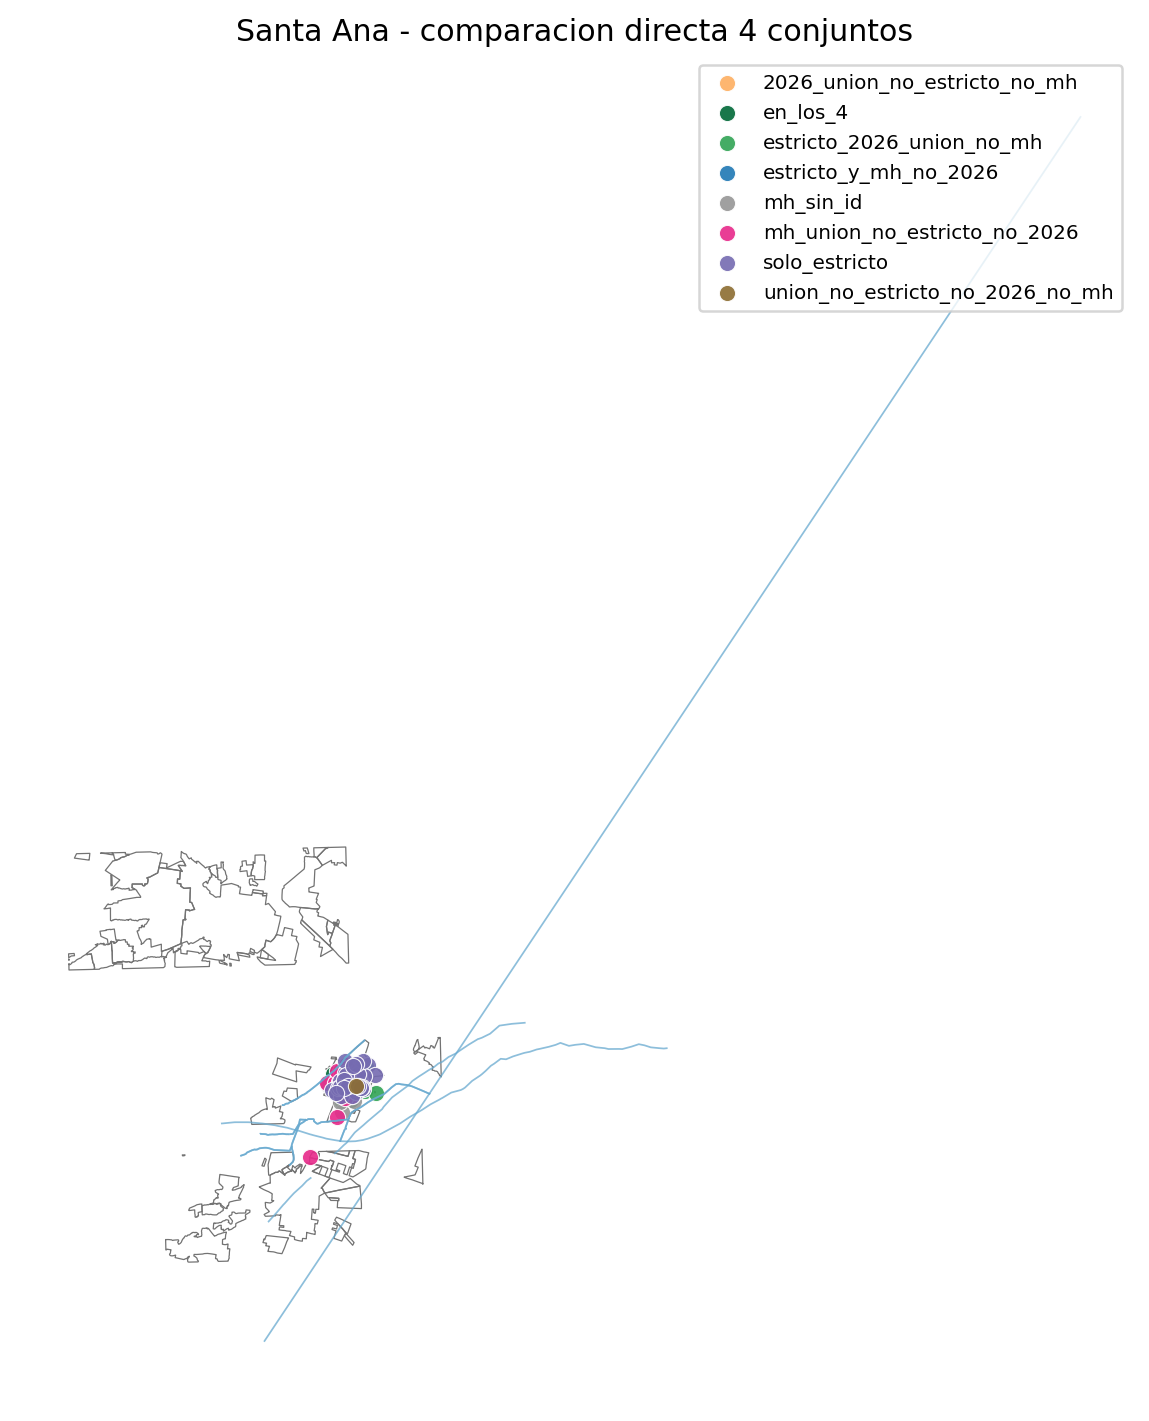
\includegraphics[width=0.95\linewidth]{../outputs/foco_textil_estricto_santa_ana_2026/mapas/mapa_comparacion_directa_4_conjuntos.png}

\caption{Comparacion directa entre foco estricto, filtrado 2026, MH y union previa.}

\end{figure}

\begin{figure}[h!]\centering

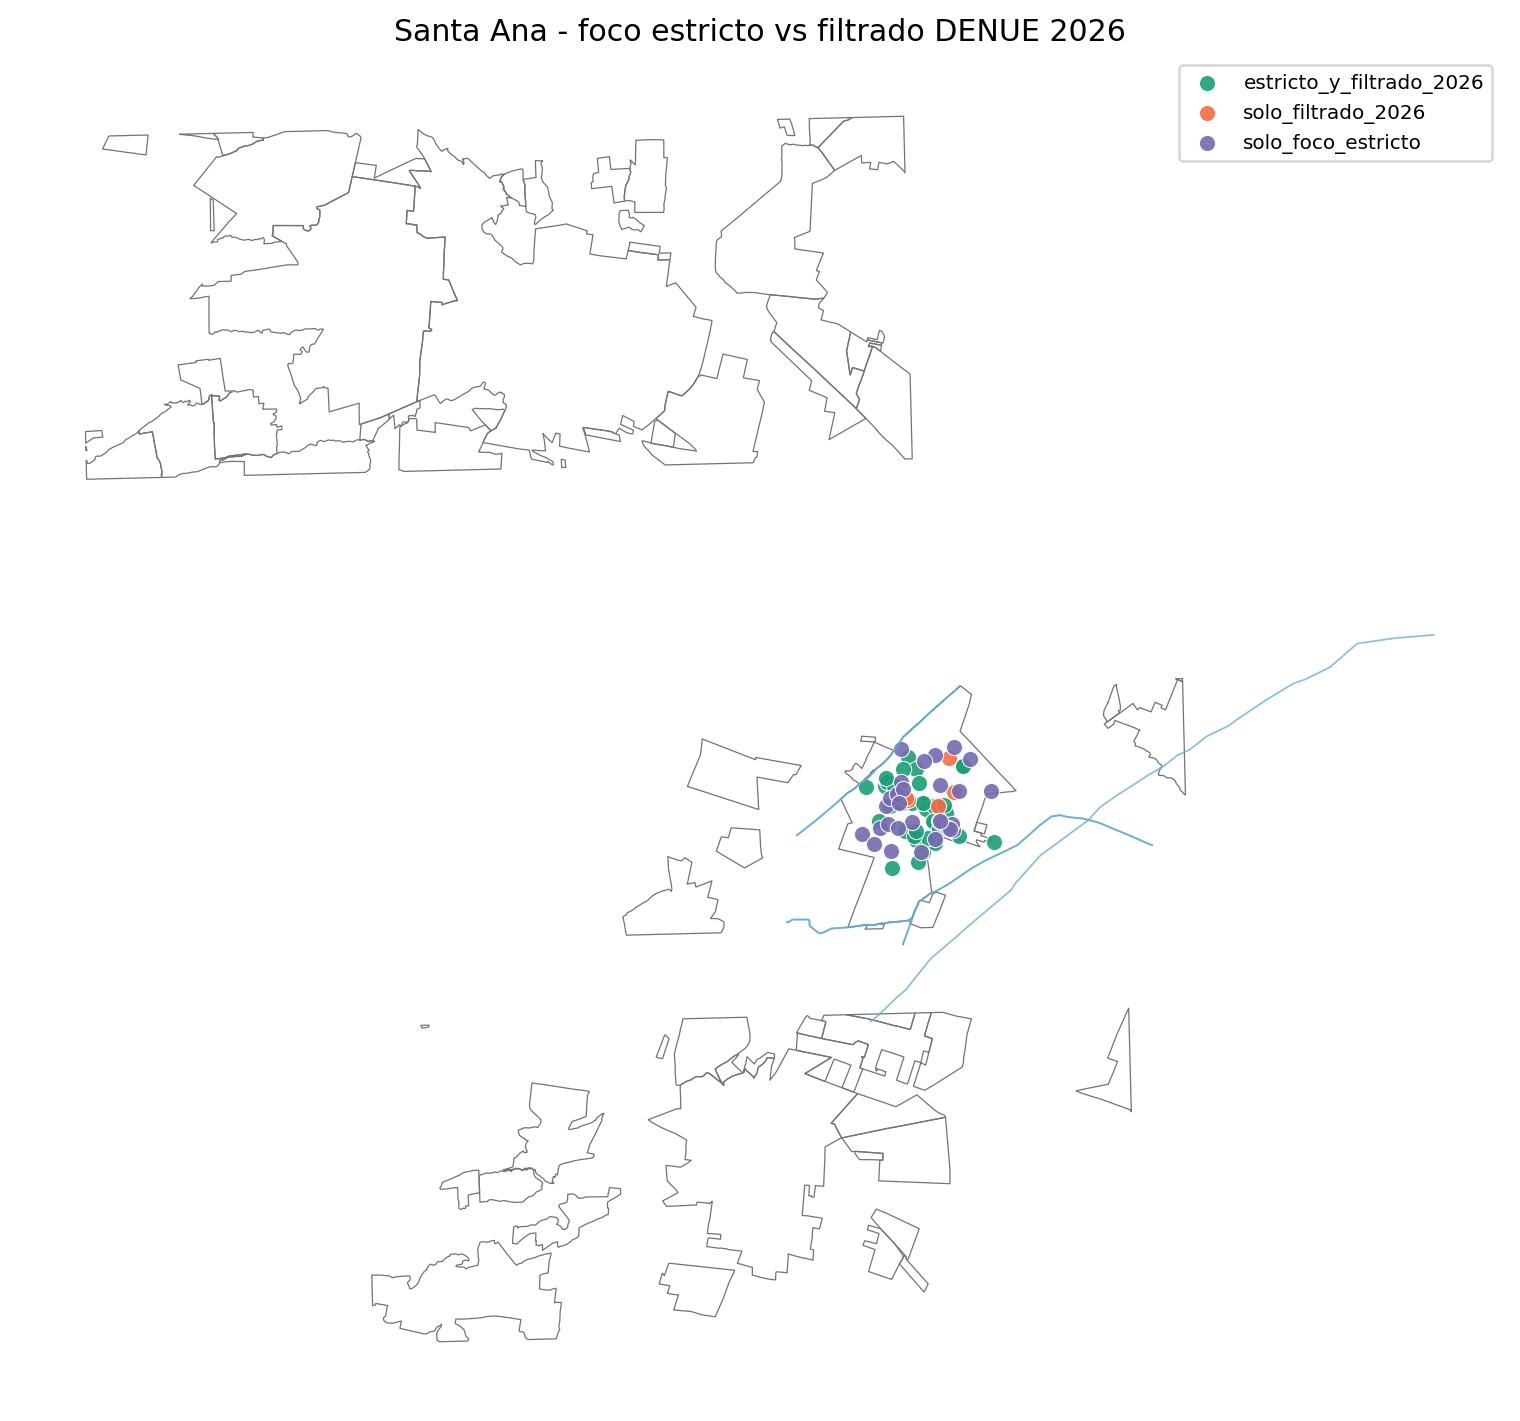
\includegraphics[width=0.95\linewidth]{../outputs/foco_textil_estricto_santa_ana_2026/mapas/mapa_foco_estricto_vs_filtrado_2026.png}

\caption{Foco estricto frente al filtrado prioritario DENUE 2026.}

\end{figure}

\begin{figure}[h!]\centering

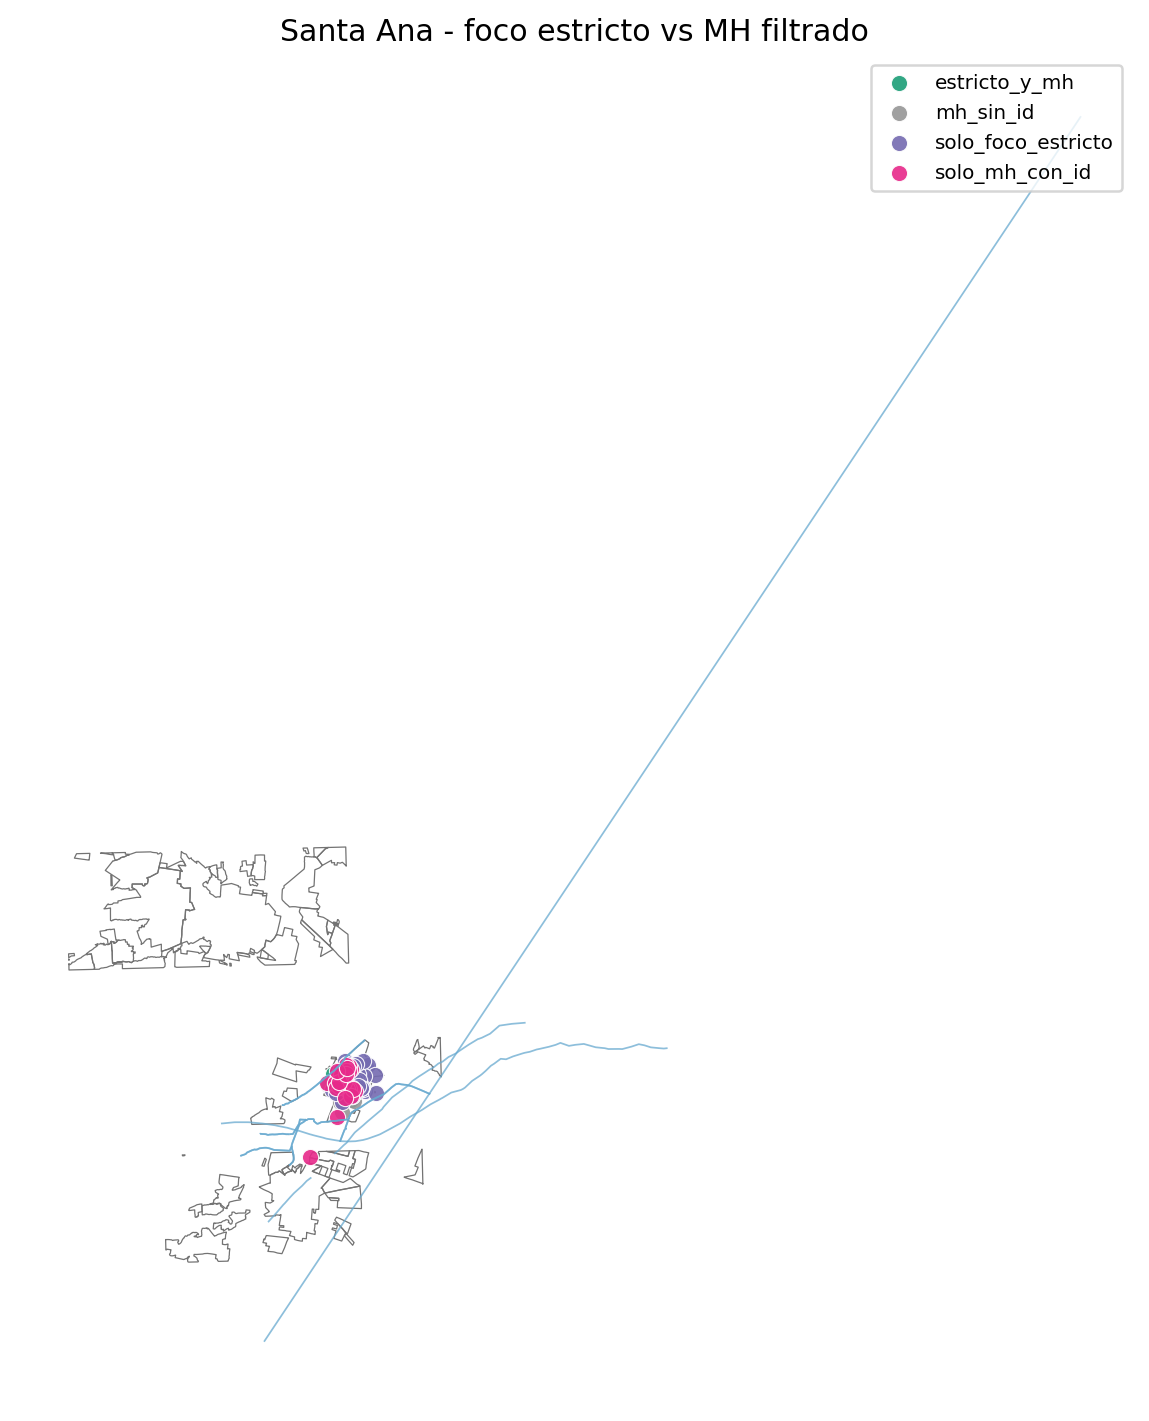
\includegraphics[width=0.95\linewidth]{../outputs/foco_textil_estricto_santa_ana_2026/mapas/mapa_foco_estricto_vs_mh_directo.png}

\caption{Foco estricto frente a MH filtrado.}

\end{figure}

\section{Conclusion operativa}

El foco estricto conserva el nucleo de establecimientos con senales mas pertinentes para auditoria ambiental de proceso textil. La capa MH filtrada coincide solo parcialmente, lo que confirma que MH usa un criterio mas amplio de talleres o maquilas. El filtrado DENUE 2026 coincide en una parte importante, pero algunos registros salen del foco estricto por ser servicios de agua, insumos, bodegas o senales no suficientemente textiles. La union previa es util como inventario de auditoria, mientras que el foco estricto es la capa recomendada para presentar un universo depurado de proceso textil.

\section{Archivos generados}

\begin{itemize}

\item \texttt{outputs/foco\_textil\_estricto\_santa\_ana\_2026/capas\_qgis/comparacion\_directa\_4\_conjuntos.gpkg}

\item \texttt{outputs/foco\_textil\_estricto\_santa\_ana\_2026/tablas/comparacion\_directa\_4\_conjuntos.csv}

\item \texttt{outputs/foco\_textil\_estricto\_santa\_ana\_2026/mapas/mapa\_comparacion\_directa\_4\_conjuntos.html}

\item \texttt{outputs/foco\_textil\_estricto\_santa\_ana\_2026/mapas/mapa\_foco\_estricto\_vs\_filtrado\_2026.html}

\item \texttt{outputs/foco\_textil\_estricto\_santa\_ana\_2026/mapas/mapa\_foco\_estricto\_vs\_mh\_directo.html}

\end{itemize}

\end{document}